\section{Implementación} \label{sec:software}

Con el objetivo de distribuir el software para múltiples plataformas a partir de la misma base de código, se emplearon lenguajes de programación web, principalmente, HTML5, JavaScript, CSS y las extensiones de estos lenguajes: TypeScript, Sass y JSX. La tecnología web tiene la ventaja de generar un software encapsulado en documentos que son compatibles con un amplio espectro de dispositivos, dado que se ejecutan en el contexto de navegadores web como Google Chrome o Mozilla Firefox, los cuales pueden ser instalados en computadoras personales, teléfonos inteligentes, \textit{Smart TVs}, \textit{Smart watches}, entre muchos otros. Por otro lado, el inconveniente que se presenta desde el punto de vista tanto comercial como de seguridad, es que el código fuente queda disponible y es accesible por parte del usuario para ser manipulado, copiado o alterado \cite{jazayeri}. En esta sección se enumeran las tecnologías utilizadas para el desarrollo de la propuesta y se describen brevemente las principales consideraciones que fueron tenidas en cuenta durante la construcción del sistema.

\subsection{Entorno de desarrollo}
El proyecto se implementó empleando a Vite\footnote{https://vitejs.dev/} como herramienta de gestión del código fuente y dependencias. Este software provee una serie de utilidades que agilizan el desarrollo del proyecto, particularmente del \textit{``front-end''}, como por ejemplo un servidor local con \textit{``hot reloading''}, un empaquetador o \textit{``bundler''} y una serie de comandos para el despliegue y testeo de la aplicación para distintos entornos.

El proyecto consta de múltiples puntos de entrada que apuntan a distintos objetivos de compilación: 1) una versión web \textit{on-line}, 2) una versión de escritorio y 3) una versión móvil. Las versiones de escritorio y móvil emplean componentes nativos de los distintos sistemas operativos, y que se acceden a través de \textit{``APIs''} tal como se describe en la sección \ref{sec:nativo}. La versión \textit{on-line} dispone de acceso limitado a ciertas herramientas y funcionalidades, para proteger recursos como \textit{API tokens} o código fuente de lógicas de negocio sensibles o que no se desea que sean accesibles por parte del usuario. Para lograr múltiples puntos de entrada en un proyecto \textit{``monorepo''}, se editaron los comandos de compilación del gestor de paquetes \textit{NPM}\footnote{https://www.npmjs.com/} indicando un archivo de configuración de Vite para cada objetivo. Este esquema permite reutilizar lógica y componentes entre las distintas versiones y mantener cada una con mínimo esfuerzo.

\subsection{Componentes nativos} \label{sec:nativo}
El esquema de desarrollo híbrido permite generar software ejecutable a partir de una aplicación web, lo que posibilita el funcionamiento de la misma de forma \textit{off-line}, de manera similar al esquema de aplicación web progresiva (PWA, por sus siglas en inglés), con la ventaja de que es posible acceder a utilidades nativas por medio de \textit{plugins} o APIs. Para lograr esto en plataformas móviles se utilizó CapacitorJS\footnote{https://capacitorjs.com/} y en el caso de sistemas operativos de escritorio como Windows o Linux, ElectronJS\footnote{https://www.electronjs.org/es/}. La versión compatible con sistemas operativos Android se puede descargar desde la tienda de aplicaciones Google Play\footnote{https://play.google.com/store/apps/details?id=com.sendevo.agrario}.

\subsection{Almacenamiento local}
Para el almacenamiento persistente de datos se emplean distintas tecnologías dependiendo del objetivo de compilación. En todos los casos se emplean representación de datos por pares clave-valor (KVP, por sus siglas en inglés).

La versiones \textit{on-line} y PWA emplean \textit{``localStorage''}, que consiste en un espacio para el almacenamiento persistente de datos mediante KVP. Este sistema está limitado a un espacio de 5 Mb, aunque puede variar dependiendo del navegador web. Para extender el almacenamiento, se incluye opcionalmente una conexión a una base de datos remota basada en el servicio de Google Firebase\footnote{https://firebase.google.com/}, que actúa como backup o sistema de sincronización de los datos de usuario entre varios dispositivos.

En el caso de las versiones nativas, se hace uso de los \textit{plugins} provistos por los distintos \textit{frameworks}, como \textit{Capacitor Storage} o \textit{FileReader}, en el caso de ElectronJS. 

\subsection{Almacenamiento distribuido} \label{sec:comunicacion}
La posibilidad de compartir información entre distintos usuarios siempre ha sido una utilidad muy requerida en la gran mayoría de los productos de software y no es diferente en el caso de las herramientas digitales para el agro \cite{davis1989,venkatesh2003,briggerman2010,michels2020}. 

El desafío que se presenta en este caso es la falta de conectividad permanente, por lo que se debe recurrir a enlaces punto a punto. Una manera para lograr este objetivo es el uso de la conectividad Bluetooth, sin embargo existen algunas limitaciones de practicidad que hacen que esta tecnología no sea muy aplicada para este propósito.

En el caso de la propuesta que se presenta en este trabajo se optó por mecanismos de comunicación empleados por aplicaciones descentralizadas. Una tecnología que resuelve la problemática de compartir información sin la participación de un intermediario es el Sistema de Archivos Interplanetario (IPFS, por sus siglas en inglés) \cite{tschorsch2022}. Para implementar el protocolo mediante tecnología web se hizo uso de la librería JS-IPFS\footnote{https://js.ipfs.tech/}, que emplea WebRTC\footnote{https://webrtc.org/} como medio de comunicación entre navegadores, permitiendo ejecutar un nodo en el contexto del navegador web. 

Existen distintas consideraciones que deben tenerse en cuenta al momento de desarrollar y utilizar sistemas de almacenamiento distribuidos, ya que implica un cambio de paradigma en lo que respecta a los aspectos que garantizan la persistencia y disponibilidad de los datos \cite{guidi2021,shen2019}. 

Si bien existen soluciones desarrolladas sobre IPFS que resuelven la implementación completa para bases de datos distribuidas, como OrbitDB\footnote{https://orbitdb.org/} o GunJS\footnote{https://gun.eco/}, para una primera versión de la propuesta presentada en este trabajo y dado que no se requieren mecanismos avanzados de sincronización de datos entre pares, se optó por el desarrollo de métodos \textit{ad-hoc}, para reducir dependencias innecesarias. Entonces, para resolver el problema de la edición colaborativa de datos que se describió en la sección \ref{sec:datos}, se ejecuta un nodo local IPFS, que en conjunto con los mecanismos de almacenamiento local, permiten acceder y compartir datos entre pares. Si bien la versión actual de la propuesta no posee esta caraterística, es posible ejecutar el nodo IPFS en segundo plano mediante una API nativa, como se presentó en \cite{cristea2020}. 

\subsection{Interfaz gráfica}
La interfaz gráfica de usuario (GUI, por sus siglas en inglés) se implementó con la ayuda de React y MUI\footnote{https://react.dev/, https://mui.com/}. Estas herramientas de código abierto proveen una lista de componentes de propósito general listos para usar, como botones, menúes, formularios, entre otros. Además se incluyó una lista de íconos predefinidos\footnote{https://react-icons.github.io/react-icons}, reduciendo el costo de diseño gráfico. 

\begin{figure}[ht]
    \hfill
    \subfigure[Edición de tarea]{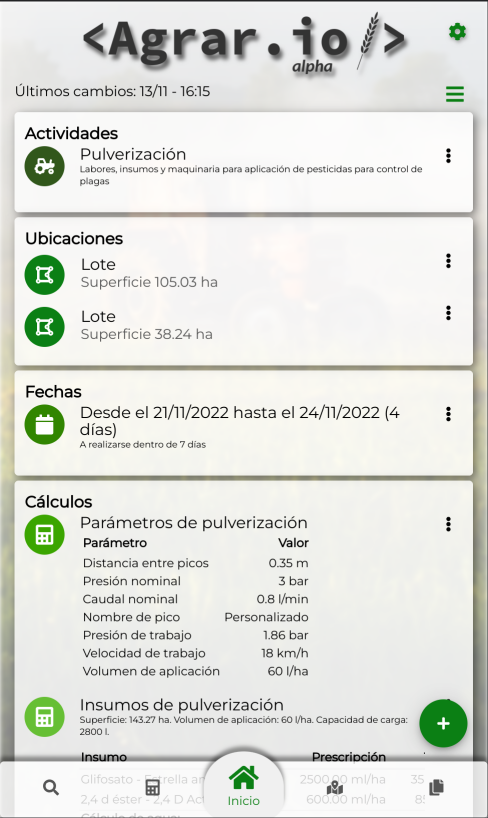
\includegraphics[width=0.3\textwidth]{imagenes/screenshot-0-lowres.png}}
    \hfill
    \subfigure[Edición de ubicaciones]{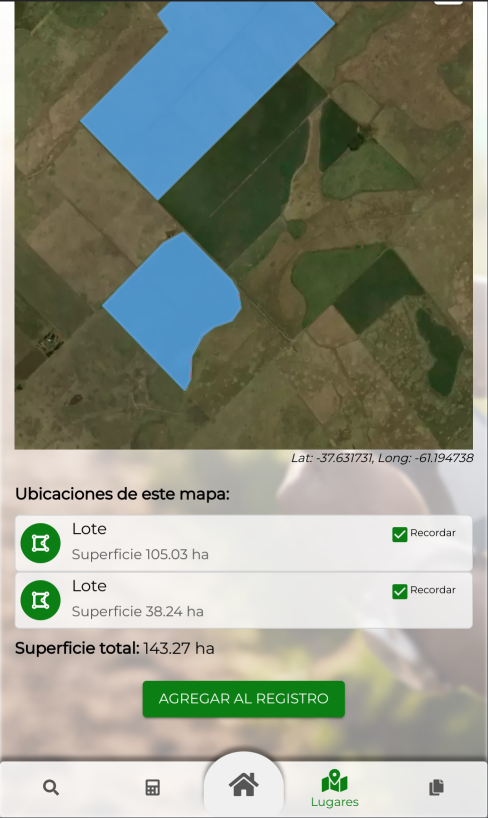
\includegraphics[width=0.3\textwidth]{imagenes/screenshot-5-lowres.png}}
    \hfill
    \subfigure[Cálculo de insumos]{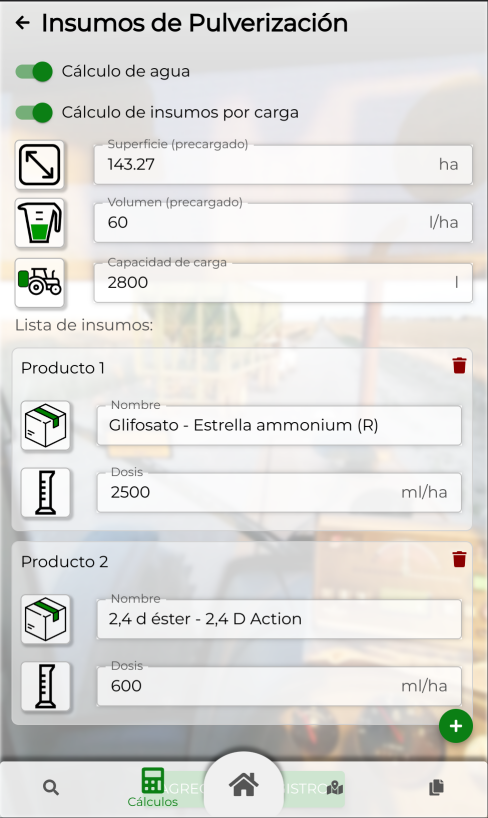
\includegraphics[width=0.3\textwidth]{imagenes/screenshot-6-lowres.png}}
    \hfill
    \caption{Capturas de pantalla de la aplicación} \label{fig:capturas}
\end{figure}

La traducción o cambio de idioma del contenido de las vistas se realiza con la ayuda del \textit{framework} de internacionalización \textit{i18next}\footnote{https://www.i18next.com/}, para el cual fueron definidos diccionarios en formato ``json'' con las traducciones de todos los términos que aparecen en la GUI. Actualmente sólo se cuenta con los idiomas español e inglés americano.

La Figura \ref{fig:capturas} muestra algunas capturas de pantalla de la aplicación móvil donde se puede observar las ventanas de edición documentos y de polígonos para lotes y a la derecha, una vista de cálculo de parámetros, particularmente de insumos de pulverización. Cada uno de estos menús posee un botón para insertar la información generada en el documento de tarea que se encuentra en edición. 


\subsection{Mapas}
Para permitir al usuario especificar ubicaciones georeferenciadas se incorpora una herramienta que facilita el dibujado de geometrías de manera gráfica sobre imágenes satelitales. De esta forma es posible ubicar marcadores, definir líneas o polígonos para indicar lotes o parcelas. Esta utilidad se implementó con la librería React-Map-GL, que emplea un servicio de MapBox\footnote{https://github.com/visgl/react-map-gl, https://www.mapbox.com/} para acceder a imágenes satelitales actualizadas. Este es un servicio gratuito siempre y cuando la cantidad de solicitudes de renderizado de mapas sea menor a una cota máxima. El formato que se utiliza para registrar las geometrías definidas por el usuario es GeoJSON\cite{geojson}, por razones de compatibilidad con el funcionamiento de MapBox y los métodos de conversión desde formatos KML o GPX, lo que facilita importar geometrías desde otras plataformas. Para los cálculos geoespaciales tales como distancias, superficies o determinación de centroides, se utilizó la librería TurfJS\footnote{https://turfjs.org/}.

\subsection{Clima y registro de variables}
La implementación actual de este software aún no cuenta con conexión a una interfaz de aplicación (API, por sus siglas en inglés) para obtener datos climáticos, pero se dispone de un formulario para el registro manual de variables definidas por el usuario y que se almacenan como parámetros, dentro de la base de datos de tareas. Esto permite realizar tareas de monitoreo o adquisición manual de datos.

Para complementar otros detalles que se quieran adicionar al registro de tareas, se dispone de un formulario para la redacción de notas de texto y también un espacio para adjuntar imágenes que se pueden cargar desde la galería de fotos del usuario o directamente capturar con la cámara del dispositivo. Todas las fotografías se codifican en \textit{base64} y se comprimen para que no superen los 100 kb en este formato, previo a su almacenamiento. 

\subsection{Generación de documentos PDF}
Esta funcionalidad se implementó con la librería PDFMake\footnote{https://pdfmake.org/} que provee un método para generar documentos en formato pdf a partir de un objeto de configuración y un arreglo de contenido. Para cada tipo de ítem descripto en la sección \ref{sec:modelo} se desarrolló un método que permite generar el bloque de contenido correspondiente a ser insertado en el documento pdf. De esta forma es posible exportar cualquier documento de la base de datos de tareas registradas por el usuario como un archivo pdf y luego ser compartido por medios externos como mensajería instantánea o correo electrónico.

Parte de la configuración propia de los documentos exportados es editable por el usuario, por ejemplo los márgenes, encabezados y pies de página, lo que permite agregar logos, membretes y personalizar el documento antes de compartirlo. Este caso de uso se aplica principalmente a empresas, contratistas o asesores que desean insertar su identidad a los documentos generados con la aplicación.
